\documentclass[11pt]{article}

\usepackage[margin=1.1in]{geometry}
\usepackage{lmodern}
\usepackage[T1]{fontenc}
\usepackage{amsmath,amssymb,amsthm}
\usepackage{booktabs}
\usepackage{listings}
\usepackage{xcolor}
\usepackage{tikz}
\usetikzlibrary{arrows.meta,positioning,fit,backgrounds,calc}
\usepackage{url}
\usepackage[colorlinks=true,linkcolor=blue!50!black,citecolor=blue!50!black,urlcolor=blue!50!black]{hyperref}
\usepackage{microtype}
\usepackage{framed}

% audience boxes: a colored left bar in the owning system's color,
% matching the code-listing aesthetic
\newenvironment{audiencebox}[1]{%
  \def\FrameCommand{{\color{#1}\vrule width 2.5pt}\hspace{9pt}}%
  \MakeFramed{\advance\hsize-\width\FrameRestore}\noindent\ignorespaces}%
  {\endMakeFramed}

% ---------------------------------------------------------------
% Color scheme.  Red = Macaulay2 (untrusted computation),
% blue = Lean (trusted verification), amber = the protocol boundary.
% Listings are color-coded by which system owns the artifact.
% ---------------------------------------------------------------
\definecolor{m2col}{RGB}{158,27,50}
\definecolor{leancol}{RGB}{28,86,178}
\definecolor{protocol}{RGB}{176,108,0}
\definecolor{okgreen}{RGB}{0,128,0}
\definecolor{warnamber}{RGB}{176,108,0}
\definecolor{badred}{RGB}{180,30,30}

\newcommand{\proved}{\textcolor{okgreen}{\code{proved}}}
\newcommand{\checked}{\textcolor{warnamber}{\code{checked}}}

\lstdefinelanguage{lean}{
  keywords={theorem,def,structure,inductive,abbrev,instance,example,by,match,with,fun,let,if,then,else,do,return,import,namespace,end,open,variable,deriving,where,noncomputable,section},
  sensitive=true, comment=[l]{--}, morecomment=[s]{/-}{-/},
  morestring=[b]",
}
\lstdefinelanguage{m2}{
  keywords={loadPackage,ideal,minors,matrix,res,assert,needsPackage,diff,flatten,for,list,comodule},
  sensitive=true, comment=[l]{--}, morestring=[b]",
}
\lstdefinestyle{leanstyle}{language=lean,
  frame=leftline, framerule=1.6pt, rulecolor=\color{leancol},
  backgroundcolor=\color{leancol!4}, keywordstyle=\bfseries\color{leancol}}
\lstdefinestyle{m2style}{language=m2,
  frame=leftline, framerule=1.6pt, rulecolor=\color{m2col},
  backgroundcolor=\color{m2col!5}, keywordstyle=\bfseries\color{m2col}}
\lstdefinestyle{jsonstyle}{
  frame=leftline, framerule=1.6pt, rulecolor=\color{protocol},
  backgroundcolor=\color{protocol!4}, keywordstyle=\bfseries}
\lstset{
  basicstyle=\ttfamily\small, keywordstyle=\bfseries,
  commentstyle=\color{gray}, columns=fullflexible,
  breaklines=true, frame=single, framerule=0.2pt, rulecolor=\color{gray!50},
  aboveskip=0.7em, belowskip=0.7em, showstringspaces=false,
  literate={∈}{{\,$\in$\,}}1 {≤}{{\,$\le$\,}}1 {→}{{\,$\to$\,}}1
    {ℚ}{{$\mathbb{Q}$\,}}1
    {∀}{{$\forall$\,}}1 {×}{{\,$\times$\,}}1 {≠}{{\,$\ne$\,}}1 {∘}{{\,$\circ$\,}}1
    {⟨}{{$\langle$}}1 {⟩}{{$\rangle$}}1 {Σ}{{$\Sigma$}}1 {∑}{{$\sum$}}1
    {⊆}{{\,$\subseteq$\,}}1 {⊕}{{\,$\oplus$\,}}1 {⁻}{{${}^-$}}1 {ᵢ}{{${}_i$}}1
    {₀}{{${}_0$}}1 {₁}{{${}_1$}}1 {₂}{{${}_2$}}1 {ₖ}{{${}_k$}}1
    {∃}{{$\exists$\,}}1 {∉}{{\,$\notin$\,}}1 {∧}{{\,$\wedge$\,}}1
    {α}{{$\alpha$}}1 {σ}{{$\sigma$}}1 {δ}{{$\delta$}}1
    {³}{{${}^3$}}1 {⁴}{{${}^4$}}1 {Φ}{{$\Phi$}}1 {ζ}{{$\zeta$}}1
    {ⱼ}{{${}_j$}}1 {ₜ}{{${}_t$}}1
}

\newtheorem{theorem}{Theorem}[section]
\newtheorem{proposition}[theorem]{Proposition}
\newtheorem{definition}[theorem]{Definition}
\newtheorem{remark}[theorem]{Remark}
\newtheorem{example}[theorem]{Example}

\newcommand{\M}{\textit{Macaulay2}}
\newcommand{\lean}{\textit{Lean}}
\newcommand{\mathlib}{\textsf{mathlib}}
\newcommand{\QQ}{\mathbb{Q}}
\newcommand{\lm}{\operatorname{lm}}
\newcommand{\code}[1]{\texttt{#1}}

\title{\textbf{M2Lean: A Certificate-Based Bridge Between\\ Macaulay2 and Lean~4}}
\author{Andrew Tawfeek\thanks{Independent researcher.
\texttt{atawfeek.math@gmail.com}.  The implementation described here
was developed with the assistance of Claude (Anthropic).  Code and all
artifacts: \url{https://github.com/andrew-tawfeek/M2Lean}.}}
\date{July 2026}

\begin{document}
\maketitle

\begin{abstract}
\M{} computes; \lean{} certifies.  M2Lean connects them through a
skeptic's contract: \M{} is an untrusted oracle whose answers must
carry \emph{certificates}---cofactors, division data, Buchberger
S-pair representations---which \lean{} re-verifies with small
checkers backed by kernel-checked soundness theorems.  We present a
versioned interchange protocol for exact commutative algebra over
$\QQ$ and prime fields, a \M{} package that exports computations with
their evidence and verifies them without leaving the \M{} session,
and a \lean{}~4 library whose accepted claims become genuine
\mathlib{} propositions.  The Gr\"obner tier is fully proved: we
formalize Buchberger's criterion in standard-representation form and
the degree-reverse-lexicographic monomial order (both absent from
\mathlib{}), so certified Gr\"obner bases and negative certificates
(non-membership via normal forms) carry kernel-checked soundness.  A
\code{by macaulay2} tactic closes ideal-membership goals by consulting
a live \M{} process and kernel-checking its answer.  A flagship
example proves the twisted cubic cone disjoint from a line over every
nontrivial commutative $\QQ$-algebra; further examples reach into
invariant theory, algebraic statistics, Galois theory (a certified
\code{Polynomial.Separable} instance), graph coloring, combinatorial
algebraic geometry, and $\mathbb{F}_{101}$.  Corrupted certificates
are rejected; continuous integration replays everything.
\end{abstract}

\section{Introduction}\label{sec:intro}

Somewhere in the literature of commutative algebra, a proof reaches a
step that reads: \emph{``a Macaulay2 computation shows that the
minimal free resolution has Betti numbers $1, 3, 2$.''}  The referee
does not re-run the computation.  The reader a decade later cannot:
the session is gone, its package versions, options, and monomial-order
conventions unrecorded.  Journals accept such sentences routinely ---
computation inside proofs is ordinary mathematics now --- and yet each
one is a small act of faith in three decades of highly optimized,
unverified C++.  The anxiety is not hypothetical, and mathematics has
already answered it once: the celebrated formalizations of the
four-color theorem~\cite{gonthier}, the Kepler
conjecture~\cite{hales-flyspeck}, and the Liquid Tensor
Experiment~\cite{scholze-liquid} were, at heart, campaigns to remove
exactly this kind of faith from exactly such computational steps.
M2Lean is a system for removing it from computational commutative
algebra --- routinely, cheaply, and without asking anyone to abandon
their tools.

The two tools in question serve different masters.  A working
algebraic geometer who wants to \emph{compute}---a Gr\"obner basis, a
free resolution, a primary decomposition---reaches for a computer
algebra system such as \M{}~\cite{M2}.  A mathematician who wants to
\emph{certify}---to produce a machine-checked proof---reaches for a
proof assistant such as \lean{}~4~\cite{lean4} with its mathematical
library \mathlib{}~\cite{mathlib}.  These ought to be two halves of
one workflow; in practice they are disconnected, because \lean{}'s
algebra library, while remarkably broad, contains almost none of the
executable machinery of computational commutative algebra, and \M{}'s
answers carry no evidence a proof assistant could accept.

M2Lean is a bridge between the two systems designed around a division
of labor rather than a translation:

\begin{center}
\begin{tabular}{ll}
\toprule
\M{} & the \emph{computational laboratory}: discovers examples,\\
     & computes bases, resolutions, invariants, decompositions\\
\lean{} & the \emph{logical authority}: fixes the mathematical meaning\\
        & of those computations and certifies conclusions\\
\bottomrule
\end{tabular}
\end{center}

The goal is not to translate \M{} source code into \lean{}, nor to
verify \M{}'s implementation.  It is to create a shared mathematical
language and a bidirectional protocol through which a computation can
cross from one system to the other \emph{without losing its meaning,
its assumptions, or its checkability}.

\paragraph{Finding is hard; checking is easy.}
The entire design rests on one asymmetry.  Deciding ideal membership
is EXPSPACE-complete in general~\cite{mayr-meyer}; Gr\"obner engines
represent decades of algorithmic engineering precisely because the
\emph{search} is expensive.  But the witness the search produces ---
cofactors expressing an element in the generators, division quotients
realizing an S-polynomial reduction --- can be verified by checking
finitely many polynomial identities, a task a patient student could
do by hand.  M2Lean asks \M{} only for what its algorithms already
possess internally (witnesses) and asks \lean{} only for what a proof
kernel is built to do (check them).  Neither system is asked to
become the other.  This is why the bridge is cheap: certified answers
in this paper cost milliseconds to re-verify and kilobytes to store
(\S\ref{sec:experiments}), while remaining checkable by any \lean{}
installation, forever, with every assumption pinned down.

\paragraph{What arrives is more than what was sent.}
A certificate crosses the bridge as arithmetic and arrives as
geometry.  In the flagship example (\S\ref{sec:flagship}), \M{}'s
witness is a two-line polynomial identity,
$1 = (-1)(xz-y^2) + (-y-1)(y-1) + x\cdot z$; the \lean{} theorem it
yields says that the cone over the twisted cubic and a line have no
common point over \emph{every} nontrivial commutative
$\QQ$-algebra --- a quantification \M{} cannot even express.  In the
Galois example (Appendix~\ref{app:more}), a two-term B\'ezout
identity arrives as \code{Polynomial.Separable}, a named concept of
the mathematical library, ready to feed into field theory.  The
bridge is not a printer: \lean{} adds generality and meaning that
\M{} does not have, and \M{} supplies discoveries that \lean{} could
not have found.

\paragraph{The skeptic's contract.}
M2Lean adopts the classical skeptical stance toward computer
algebra~\cite{harrison-thery}: \M{} is treated as an untrusted oracle.
A result is never accepted because \M{} printed \code{true}; it is
accepted only when \M{} supplies \emph{evidence}---cofactors
expressing an element in terms of generators, change-of-basis data,
division quotients for S-polynomials---and a small \lean{} checker
verifies that evidence.  For the core checkers we prove soundness
theorems in \lean{}: if the checker accepts, a genuine \mathlib{}
proposition holds.  A defect anywhere in \M{}, in the bridge code, or
in the serialization can cause spurious \emph{rejection}, but never a
false theorem.

\paragraph{Contributions.}
This paper describes the design and a complete working vertical slice
of the bridge, the \emph{M2Lean Bridge Core}:

\begin{enumerate}
\item \textbf{A versioned interchange protocol} (\S\ref{sec:protocol})
  for exact commutative algebra over $\QQ$ and prime fields:
  polynomial rings with normatively specified monomial orders, ideals,
  matrices, graded free modules, and seven kinds of \emph{claims with
  evidence}, including negative certificates.  Canonical forms are
  strict enough that equality of encodings is structural, and
  consumers reject rather than repair.
\item \textbf{A \M{} bridge package} (\S\ref{sec:m2}) that exports
  objects, produces certificates from public \M{} interfaces
  (including S-pair evidence from an explicit division algorithm),
  and closes the loop in-session: \code{verifyWithLean~D} spawns the
  \lean{} verifier on the current document and displays colored
  per-claim verdicts without leaving \M{}.
\item \textbf{A \lean{}~4 library} (\S\ref{sec:lean}) with an
  executable sparse model over any coefficient field (instantiated at
  $\QQ$ and \code{ZMod p}), a strict protocol validator, certificate
  checkers, and machine-checked soundness theorems producing genuine
  \mathlib{} propositions.
\item \textbf{A formalized Gr\"obner tier}
  (\S\ref{sec:groebner}): Buchberger's criterion in
  standard-representation form (\code{buchberger\_criterion}) and the
  degree-reverse-lexicographic order as a \mathlib{}
  \code{MonomialOrder} (\code{degRevLex}), both new formalizations and
  natural \mathlib{} upstream candidates, plus the bridge lemmas
  connecting them to the executable checker.  Gr\"obner and
  non-membership certificates over GRevLex are \proved{}, not merely
  \checked{}.
\item \textbf{A \code{by macaulay2} tactic} (\S\ref{sec:tactic}):
  ideal-membership goals are discharged by consulting a live \M{}
  subprocess and kernel-checking the returned certificate at
  elaboration time.
\item \textbf{A flagship theorem and cross-area examples}
  (\S\ref{sec:flagship}, Appendix~\ref{app:more}): certified
  disjointness of the twisted cubic cone and a line over every
  nontrivial commutative $\QQ$-algebra; a kernel-checked
  \code{Polynomial.Separable} for $X^4+1$ over $\QQ$; Gr\"obner, membership, and
  non-membership over $\mathbb{F}_{101}$; and more --- with an axiom
  audit showing no additions to \lean{}'s standard three axioms.
\item \textbf{Adversarial testing and continuous integration}
  (\S\ref{sec:experiments}): mutated real certificates and malformed
  documents are rejected with failure-class diagnostics; a GitHub
  Actions pipeline regenerates every \M{} document, rebuilds the
  \lean{} library (exercising the tactic against a live \M{}), and
  replays all 19 checks and the axiom audit on every push.
\end{enumerate}

\paragraph{How to read this paper.}
Readers coming from \M{} may prefer \S\ref{sec:whatbuys},
\S\ref{sec:m2}, the flagship walk-through (\S\ref{sec:flagship}), and
the condensed examples of Appendix~\ref{app:more}; none of these
require reading \lean{}.  Readers coming from \lean{} will find the
mathematical content in \S\ref{sec:lean}--\S\ref{sec:tactic},
especially the Gr\"obner formalization (\S\ref{sec:groebner}).
Readers inclined to trust neither system should start with the trust
model (\S\ref{sec:trust}) and the adversarial evaluation
(\S\ref{sec:experiments}).

Everything is open source; the repository contains the protocol
specification, both implementations, all fixtures, and scripts that
reproduce every claim in this paper~\cite{m2lean-repo}.

\section{What this buys you}\label{sec:whatbuys}

\begin{audiencebox}{m2col}
\textbf{\textcolor{m2col}{If you use Macaulay2.}}\quad
Your computations become citable.  A session that today ends with a
printed Betti table can end with one extra call,
\code{verifyWithLean D}, and produce a certificate that any \lean{}
installation --- a referee's, a reader's, one running twenty years
from now --- can re-check, with the coefficient field, monomial
order, grading, and package versions pinned down machine-readably.
You never write a line of \lean{}.  The discipline pays even before
verification: making certificates exportable forced exact answers to
questions the ecosystem usually leaves implicit (which GRevLex
tie-break convention is in force; what the division algorithm
guarantees about its quotients), and the shared adversarial fixtures
would catch any future drift.  And the statuses are honest: a
computation is reported as \emph{computed}, \checked{}, or \proved{},
never a conflation of the three.
\end{audiencebox}

\begin{audiencebox}{leancol}
\textbf{\textcolor{leancol}{If you use Lean.}}\quad
Thirty years of computational commutative algebra become available to
your proofs without anyone reimplementing them.  You do not need a
verified Gr\"obner \emph{engine} to use a Gr\"obner basis: you need a
witness and a checker, and the checker's soundness theorem makes the
result a genuine \mathlib{} proposition --- here, span membership,
ideal equality, non-membership, and vanishing compositions, consumed
by ordinary theorems with no new axioms and no \code{sorry}.  The
bridge is also a formalization engine rather than a bypass:
Buchberger's criterion and the degree-reverse-lexicographic order
entered \lean{} \emph{because} the checker demanded them
(\S\ref{sec:groebner}), and both are stated against \mathlib{}'s own
\code{MonomialOrder} theory for upstreaming.  At the ergonomic end,
\code{by macaulay2} (\S\ref{sec:tactic}) makes the round trip a
single tactic call.
\end{audiencebox}

\section{Related work}\label{sec:related}

Skeptical combination of proof assistants and computer algebra goes
back to Harrison and Th\'ery's HOL--Maple bridge~\cite{harrison-thery},
which introduced the pattern we follow: let the CAS find an object
that is expensive to discover but cheap to check (a factorization, an
antiderivative), and re-verify it in the prover.  Delahaye and
Mayero connected Coq to Maple for field
simplification~\cite{delahaye-mayero}, and Kaliszyk and Wiedijk
prototyped a full CAS on top of HOL Light~\cite{kaliszyk-wiedijk}.
Within \lean{}, the \code{linear\_combination}
tactic~\cite{linear-combination} checks exactly the kind of cofactor
certificate our membership checker consumes, and
\code{polyrith}~\cite{polyrith} obtains those cofactors by calling an
external Gr\"obner engine---a special case of the M2Lean pattern,
built directly into a tactic.  M2Lean generalizes this from single
tactic calls to a versioned, provenance-carrying protocol spanning
objects (rings, ideals, matrices, complexes) and claim families, with
an explicitly stratified trust model.

On the formalization side, Buchberger's algorithm was verified in Coq
by Th\'ery~\cite{thery-buchberger} and Gr\"obner theory is developed
in Isabelle/HOL~\cite{divason-groebner}; \mathlib{} had no comparable
development, a gap this work partially closes with a proof of
Buchberger's criterion and the degree-reverse-lexicographic order
(\S\ref{sec:groebner}), stated against \mathlib{}'s
\code{MonomialOrder} theory for upstreaming.  CoqEAL~\cite{coqeal} refines abstract algebraic structures to
efficient executable ones inside the prover; M2Lean is complementary,
keeping the heavy computation outside the prover and importing only
evidence.  Certificate-based cooperation is also standard practice in
SMT proof reconstruction~\cite{smt-certificates} and in
sums-of-squares certificates for nonlinear
arithmetic~\cite{harrison-sos}; M2Lean can be read as bringing that
discipline to computational commutative algebra, where the natural
certificates are cofactors, syzygies, and division data~\cite{clo,
becker-weispfenning}.

\section{Architecture and trust model}\label{sec:trust}

\subsection{Four layers}

\begin{center}
\begin{tabular}{ll}
\toprule
layer & realization \\
\midrule
interchange representation & \code{protocol/SPEC.md}, JSON schema, fixtures \\
semantics & \lean{}: sparse model $\to$ \code{MvPolynomial (Fin n) $\QQ$} \\
claims and certificates & \lean{} checkers $+$ soundness theorems \\
user-facing integrations & \M{} package; \code{m2lean-check} CLI \\
\bottomrule
\end{tabular}
\end{center}

A document travels left to right: \M{} exports objects and claims,
\lean{} parses and \emph{validates} (arities, canonical scalars,
dependency order, dimension checks---rejecting, never repairing), then
runs one checker per claim and emits a verification report; claims
whose checkers carry soundness theorems can additionally be consumed
by \lean{} theorem files through the kernel
(Figure~\ref{fig:flagship} traces one such trip end to end).  Parsing
is not proof: the semantics layer is what turns byte-level checks
into mathematics.

Throughout the paper, code listings are color-coded by which side of
the trust boundary owns the artifact:
\textcolor{m2col}{\textbf{red}} for \M{} input (untrusted
computation and evidence generation),
\textcolor{protocol}{\textbf{amber}} for protocol documents (the data
crossing the boundary), and \textcolor{leancol}{\textbf{blue}} for
\lean{} (validation, checking, and theorems).

\subsection{Trusted and untrusted}

The trusted base consists of the \lean{} kernel, the definitions
giving protocol objects mathematical meaning (the sparse model and its
interpretation), the statements of the soundness theorems, and
\mathlib{} itself.  Explicitly untrusted: all of \M{} (engine,
interpreter, our package), all serialization and transport, every
field of every document including provenance, and generated \lean{}
syntax prior to kernel checking.  Checkers may not use
\code{native\_decide}; certificate checks in theorem files run
through the kernel (\code{decide +kernel}).

\subsection{Assurance levels}

Every accepted claim carries one of four levels, and the distinction
is preserved end to end---in the checker code, in the CLI report, and
in which claims example theorems are permitted to consume:

\begin{center}
\begin{tabular}{lp{0.72\textwidth}}
\toprule
\textcolor{gray}{\code{transported}} & object parsed and validated; nothing checked \\
\textcolor{gray!30!black}{\code{reproduced}} & computation re-run and matched; no certificate \\
\checked{} & certificate verified by an executable checker whose
mathematical soundness is cited but not yet formalized \\
\proved{} & as \checked{}, plus a kernel-checked soundness
theorem: acceptance \emph{implies} the \mathlib{} proposition \\
\bottomrule
\end{tabular}
\end{center}

In the current implementation, polynomial identity, ideal membership,
span inclusion, chain-complex composition, Gr\"obner bases, and
non-membership are \proved{} (the latter two over GRevLex, \M{}'s
default order; their Lex instances remain \checked{} until the Lex
agreement lemmas are formalized); graded complexes are \checked{}.
Claims are checked in the coefficient field their ring declares:
$\QQ$ or, for \code{PrimeField p} documents, \code{ZMod p}.  We regard
surfacing this distinction as a design contribution rather than a
confession: systems that blur ``the checker ran'' and ``the theorem
holds'' invite exactly the silent failures a bridge like this exists
to eliminate.

\section{The interchange protocol}\label{sec:protocol}

The protocol (currently version 0.2.0, the string consumers refuse
to mismatch) deliberately covers a small, exactly
specified fragment: coefficients in $\QQ$ (reduced fractions of
decimal strings; JSON numbers are never used for mathematical data)
or $\mathbb{F}_p$ ($p$ verified prime by the consumer); multivariate
polynomial rings with positional variable identity and one of two
normatively defined monomial orders (\code{Lex} and \code{GRevLex},
\M{}'s default); sparse polynomials in canonical form (nonzero
reduced coefficients, exact arity, strictly decreasing terms); ideals;
matrices; and graded free modules $\bigoplus_j R(-d_j)$.

Canonicality is strict enough that equality of encoded polynomials is
structural equality, which is the base of every checker, and it is
enforced, not assumed: a document whose terms are misordered for the
\emph{declared} order is rejected.  This addresses a classical source
of silent cross-system corruption---graded reverse lexicographic
order alone admits several incompatible textbook conventions---by
making the definitions normative in the specification and testing
both implementations against shared adversarial fixtures ordered
differently under \code{Lex} and \code{GRevLex}.

A \emph{claim} is a proposition about previously introduced objects
plus evidence addressed to a specific checker:

\begin{center}
\small
\begin{tabular}{lll}
\toprule
claim kind & proposition & evidence \\
\midrule
\code{PolynomialIdentity} & $\mathit{lhs} = \mathit{rhs}$ & none (normalization) \\
\code{IdealMembership} & $f \in (g_1,\dots,g_k)$ & cofactors $c_i$ with $f = \sum c_i g_i$ \\
\code{SpanInclusion} & $I \subseteq J$ & a cofactor row per generator \\
\code{GroebnerBasis} & $G$ is a GB of $I$ & span witnesses both ways $+$ \\
& & S-pair standard representations \\
\code{NonMembership} & $f \notin I$ & division data vs.\ a certified GB: \\
& & $f = \sum q_k b_k + r$, $r \neq 0$ reduced \\
\code{ChainComplex} & $d_i \circ d_{i+1} = 0$ & none (matrix arithmetic) \\
\code{GradedComplex} & the above, graded & none (homogeneity checks) \\
\bottomrule
\end{tabular}
\end{center}

Documents also carry provenance---producer versions, algorithm names,
determinism flags---which is displayed for reproducibility but never
influences acceptance.  The verifier answers with a report document
whose failure messages distinguish parse, structural, and
verification failures.

The most interesting evidence format is the Gr\"obner one.  For every
pair $i<j$ of basis elements whose leading monomials are not coprime,
the producer must supply quotients $q_1,\dots,q_r$ such that
\[
  S(b_i,b_j) \;=\; \sum_k q_k\, b_k,
  \qquad
  \lm(q_k b_k) \,\preceq\, \lm\bigl(S(b_i,b_j)\bigr) \text{ whenever } q_k \neq 0,
\]
i.e.\ a \emph{standard representation}, for \emph{every} pair
(coprime pairs may not be omitted: this keeps the soundness proof
within the standard-representation criterion, without Buchberger's
first criterion).  By Buchberger's criterion in
standard-representation form~\cite[Thm.~5.64]{becker-weispfenning}%
~\cite{buchberger,clo}, verifying these identities and bounds (plus
the two span inclusions relating $G$ to the input generators)
establishes that $G$ is a Gr\"obner basis.  The point of this format
is that the checker never runs Buchberger's algorithm: it only checks
polynomial identities and monomial comparisons, both of which reduce
to the structural equality of canonical forms.  Since the criterion
itself is now formalized (\S\ref{sec:groebner}), this implication is
no longer a citation but a kernel-checked theorem.

Negative certificates ride on positive ones: a \code{NonMembership}
claim references a \code{GroebnerBasis} claim in the same document and
supplies division data with a nonzero remainder no term of which is
divisible by a basis leading monomial.  Its soundness genuinely
\emph{requires} the Gr\"obner property --- a reduced nonzero remainder
refutes membership only against a true Gr\"obner basis --- which is
why this claim kind exists at the \proved{} level only on the
strength of the Buchberger formalization.

\section{The Macaulay2 bridge package}\label{sec:m2}

The package \code{m2/M2Lean.m2} exports objects and generates
certificates using public \M{} interfaces.  From the user's point of
view, encoding mathematics for the bridge is ordinary \M{}: one
builds rings and ideals as usual, then attaches claims to a document
and writes it out.  A complete session certifying a membership looks
like this:

\begin{lstlisting}[style=m2style]
loadPackage "M2Lean";
R = QQ[x,y];
I = ideal(x+y, x-y);                        -- the mathematics, as usual
D = newM2LeanDocument "session-1";
membershipClaim(D, "mem1", x^3 + y^3, I);   -- computes the cofactors
writeM2LeanDocument(D, "session-1.json");   -- crosses the boundary
\end{lstlisting}

\noindent
The loop closes without leaving the session:

\begin{lstlisting}[style=m2style]
verifyWithLean D
-- m2lean-check report for document session-1:
--   mem1: accepted [proved]  element lies in the ideal
\end{lstlisting}

\noindent
\code{verifyWithLean} writes the document to a temporary file, spawns
the Lean verifier as a subprocess, parses the report, and displays
colored per-claim verdicts (green \code{proved}, amber \code{checked},
red rejections), returning the parsed report for programmatic use.

\code{membershipClaim} silently does the interesting work: it divides
the element against the ideal's Gr\"obner basis, extracts cofactors,
re-checks the identity, and serializes everything---generators,
element, evidence, monomial order, provenance---in the canonical
forms of \S\ref{sec:protocol}.  Because everything the package
produces is re-verified, it may freely use \M{}'s untrusted machinery:
membership cofactors come from matrix division \code{f // gens I}
against \M{}'s internal Gr\"obner engine, and basis conversion
witnesses likewise.  The one place where honesty about \emph{how} a
result was obtained matters is the S-pair evidence: \M{}'s engine
does not expose its reduction traces, so the package re-derives the
quotients with an explicit textbook division algorithm (twenty lines
of \M{} code) whose loop invariant guarantees the
standard-representation bound that the protocol demands.  This is a
small instance of a phenomenon we expect to recur: \emph{certificate
export forces implicit algorithmic guarantees to become explicit},
and occasionally forces recomputation in a shape that carries its own
correctness evidence.

One subtlety deserves record.  \M{} keeps polynomials sorted in the
ring's monomial order, so canonical export is free---but only after
the bridge verifies that \M{}'s order conventions agree with the
protocol's normative definitions.  Our test suite pins this down
empirically (e.g.\ $x + y^2z$ must serialize as $[x,\,y^2z]$ under
\code{Lex} and $[y^2z,\,x]$ under \code{GRevLex}), and the shared
fixtures would catch any drift on either side.

\section{The Lean library}\label{sec:lean}

\subsection{An executable model and its interpretation}

The computational heart is a deliberately small sparse model,
parameterized over the coefficient field (instantiated at $\QQ$ for
\code{RationalField} documents and \code{ZMod p} for
\code{PrimeField} documents, after the verifier confirms primality
and synthesizes the field instance):
\begin{lstlisting}[style=leanstyle]
structure STerm (α : Type*) where
  coeff : α
  exps  : List Nat      -- positional; entries beyond the end are 0
abbrev SPoly (α : Type*) := List (STerm α)
\end{lstlisting}
with executable normalization (sort by a fixed total comparator, then
merge equal exponent vectors and drop zeros, with trailing-zero
trimming so that paddings of the same monomial coincide), ring
operations on raw term lists, and the two protocol monomial orders.
All recursion is structural, for a reason that becomes visible later:
well-founded recursion does not reduce definitionally, and these
functions must run \emph{inside the kernel}.

The semantics is a function
\code{toMv n : SPoly $\to$ MvPolynomial (Fin n) $\QQ$}
interpreting a term list as a sum of monomials, together with a
lemma suite proved once and for all: \code{toMv} commutes with
concatenation, term-wise product, permutation, merging, and
normalization.  The payoff is the soundness of the two executable
predicates every checker is built from:
\begin{lstlisting}[style=leanstyle]
theorem polyEq_sound   (h : polyEq p q = true)     : toMv n p = toMv n q
theorem polyIsZero_sound (h : polyIsZero p = true) : toMv n p = 0
\end{lstlisting}

\subsection{Checkers and soundness theorems}

Checkers are Boolean functions on plain sparse data---independent of
the protocol AST, so the soundness theorems apply to them directly.
Representative statements (all \code{sorry}-free, all checked by the
kernel):

\begin{lstlisting}[style=leanstyle]
theorem checkMembership_sound
    (h : checkMembership f gs cs = true) :
    toMv n f ∈ Ideal.span {p | p ∈ gs.map (toMv n)}

theorem checkSpanInclusion_sound
    (h : checkSpanInclusion src tgt rows = true) :
    spanOf n src ≤ spanOf n tgt

theorem checkComplexPair_sound
    (h : checkComplexPair r m c A B = true) :
    toMatrix n r m A * toMatrix n m c B = 0

theorem no_common_zero
    (h : checkMembership onePoly gs cs = true)
    {K : Type*} [CommRing K] [Nontrivial K] [Algebra ℚ K]
    (pt : Fin 4 → K)
    (hv : ∀ g ∈ gs, aeval pt (toMv n g) = 0) : False
\end{lstlisting}

The last theorem is the abstract half of the flagship: a certificate
that $1 = \sum c_i g_i$ makes the span the unit ideal, and the unit
ideal has no common zero in any nontrivial commutative
$\QQ$-algebra---the certificate refutes points valued in every field
extension at once, which is exactly the content usually delivered by
the Nullstellensatz but obtained here by pure algebra from an
explicit witness.

The Gr\"obner checker \code{checkGroebner} verifies S-pair coverage,
each standard representation with its leading-monomial side
conditions, and both span inclusions.  The implication ``criterion
verified $\Rightarrow$ Gr\"obner basis'' is not cited here but
proved: \S\ref{sec:groebner} describes the formalization that puts
these claims at the \proved{} level --- for every certificate ever
produced, with no change to \M{} or the protocol.

\subsection{Kernel-checked certificate consumption}

The CLI accepts documents at runtime, but example \emph{theorems}
embed certificate data as literals (generated deterministically from
the JSON by a checked-in script) and verify them by kernel reduction:
\begin{lstlisting}[style=leanstyle]
theorem certificate_checks :
    checkMembership onePoly gens cofactors = true := by decide +kernel
\end{lstlisting}
Two implementation notes may save others time.  First, any
well-founded recursion in a checker silently blocks such kernel
evaluation; our merge step is a structural \code{foldr} for exactly
this reason.  Second, \code{Rat} arithmetic does not reduce in the
elaborator's evaluator but does in the kernel (which has fast
arbitrary-precision arithmetic including \code{Nat.gcd}), so
\code{decide +kernel} rather than plain \code{decide} is required.

\section{The formalized Gr\"obner tier}\label{sec:groebner}

The Gr\"obner checker is not merely executable: its acceptance
\emph{implies} the Gr\"obner property by a kernel-checked proof.
Three formalizations were required, none previously available in
\mathlib{}.

\paragraph{Buchberger's criterion.}
We prove the standard-representation form of Buchberger's
criterion~\cite{buchberger,becker-weispfenning} over an arbitrary
\mathlib{} \code{MonomialOrder} and field:

\begin{lstlisting}[style=leanstyle]
theorem buchberger_criterion
    (hb : ∀ i, b i ≠ 0)
    (hS : ∀ i j, HasStdRep m b (sPoly m (b i) (b j)))
    (hf : f ∈ Ideal.span (Set.range b)) (hf0 : f ≠ 0) :
    ∃ i, m.degree (b i) ≤ m.degree f
\end{lstlisting}

\noindent
The proof is the classical one, mechanized: pick a representation of
`f` minimizing (by well-foundedness of the order) the largest product
degree $\delta$; if $\delta$ exceeds $\deg f$, the top-degree layer
cancels and is rewritten through S-polynomial standard
representations — a cancellation lemma proved by strong induction on
the size of the layer — yielding a representation with smaller
$\delta$.  Verified Buchberger developments exist in
Coq~\cite{thery-buchberger} and Isabelle~\cite{divason-groebner};
this appears to be the first in \lean{}, and it is deliberately
stated against \mathlib{}'s own \code{MonomialOrder}/\code{degree}
theory so it can be upstreamed next to \code{MonomialOrder.div}.

\paragraph{The degree-reverse-lexicographic order.}
\mathlib{} provides \code{lex} and \code{degLex}, but not \M{}'s
default order.  We construct \code{MonomialOrder.degRevLex} as a type
synonym ordered by total degree, ties broken by the \emph{order dual}
of \mathlib{}'s colexicographic comparison.  One subtlety deserves
record: unlike \code{degLex}, whose tie-break order is itself
well-founded, plain reverse-lexicographic comparison is \emph{not}
($1 \succ x_0 \succ x_0^2 \succ \cdots$), so well-foundedness cannot
be inherited componentwise.  It holds anyway because degrees are
non-increasing along a descending chain and, over finitely many
variables, only finitely many exponent vectors exist below a given
degree --- which is why \code{degRevLex} requires \code{[Finite\,$\sigma$]},
a hypothesis \code{degLex} does not need.

\paragraph{The bridge, and checkers that check what the proof needs.}
Connecting the executable checker to the abstract criterion requires
agreement lemmas --- the byte-level comparator on exponent lists
computes exactly the \code{degRevLex} relation on interpreted
monomials --- and a \emph{lead bridge}: the head of the sorted
normalization is the abstract leading term.  The latter would need a
formal theory of sorting-with-merging; instead, the checker was
refined to \emph{certify} the facts the proof needs.  A new
\code{leadOK} check asserts, decidably, that the head strictly
dominates every other term; soundness then consumes the check rather
than a meta-theorem about the sorting algorithm.  This ``check what
the proof needs'' pattern kept the trusted development hundreds of
lines smaller, at zero cost on honest certificates.  The final
statements:

\begin{lstlisting}[style=leanstyle]
theorem checkGroebner_sound
    (h : checkGroebner n .grevlex gens basis bc gc sps = true) :
    spanOf n gens = spanOf n basis ∧
    ∀ f ∈ spanOf n basis, f ≠ 0 →
      ∃ b ∈ basis, (grevlexOrder n).degree (toMv n b) ≤
        (grevlexOrder n).degree f

theorem checkNonMembership_sound
    (hgb : checkGroebner n .grevlex gens basis bc gc sps = true)
    (hnm : checkNonMembership n .grevlex basis f quots r = true) :
    toMv n f ∉ spanOf n basis
\end{lstlisting}

\noindent
Both hold over any coefficient field, so they apply verbatim to
$\mathbb{F}_p$ documents.  The second is the promised negative
certificate: division data with a nonzero reduced remainder refutes
membership --- \emph{only} against a proved Gr\"obner basis, which is
why it ships in the same section.  Certificates over \code{Lex} rings
remain at \checked{} until the (entirely analogous) Lex agreement
lemmas are formalized; the assurance level is computed per order and
displayed per claim.

\section{The \code{by macaulay2} tactic}\label{sec:tactic}

The architecture compresses into a single tactic call:

\begin{lstlisting}[style=leanstyle]
def f : SPoly ℚ := [⟨1, [3, 0]⟩, ⟨1, [0, 3]⟩]          -- x³ + y³
def gs : List (SPoly ℚ) :=
  [[⟨1, [1, 0]⟩, ⟨1, [0, 1]⟩], [⟨1, [1, 0]⟩, ⟨-1, [0, 1]⟩]]

example : toMv 2 f ∈ spanOf 2 gs := by macaulay2
\end{lstlisting}

\noindent
The tactic reflects the goal's sparse data, writes a \M{} session
requesting a membership certificate, runs \code{M2 --script} as a
subprocess, parses the returned protocol document with the M2Lean
parser, embeds the cofactors as literals, and closes the goal with
\code{checkMembership\_sound} applied to a kernel-checked run of the
certificate checker.  The trust story is unchanged: \M{}'s answer is
data, not authority --- a wrong answer fails the kernel check and the
tactic reports an error; it can never prove a falsehood.  The demo
file above is built in continuous integration, so every CI run
exercises a live \lean{}-to-\M{} round trip at elaboration time.
This prototype handles ground membership goals; goal reflection for
symbolic polynomials (via \code{ring\_nf}-style normalization, as in
\code{polyrith}~\cite{polyrith}) is the natural next step.

\section{The flagship example}\label{sec:flagship}

The example is chosen to be mathematically recognizable, small enough
for continuous integration, and structured so that both systems are
essential (cf.~\cite{eisenbud}).  Let
$R = \QQ[x,y,z,w]$ and let
\[
I \;=\; \bigl(xz - y^2,\; xw - yz,\; yw - z^2\bigr)
\]
be the ideal of $2\times 2$ minors of
$\left(\begin{smallmatrix} x & y & z\\ y & z & w \end{smallmatrix}\right)$,
cutting out the cone over the twisted cubic curve.  Let
$L = V(y-1,\, z,\, w)$ be the line $\{(t,1,0,0)\}$.
Figure~\ref{fig:flagship} traces the artifacts through the pipeline;
the remainder of this section walks the same path in detail.

\begin{figure}[t]
\centering
\resizebox{\textwidth}{!}{%
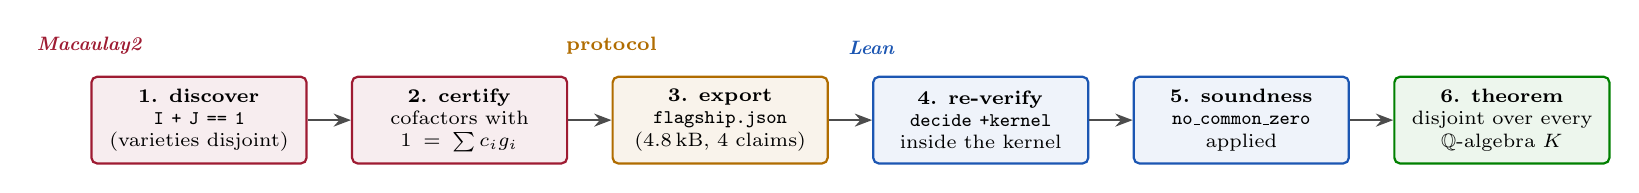
\begin{tikzpicture}[
  font=\scriptsize,
  node distance=3mm and 5.5mm,
  stage/.style={draw, rounded corners=2pt, align=center, inner sep=4pt,
               minimum height=11mm, text width=24.5mm},
  m2s/.style={stage, draw=m2col, fill=m2col!8, thick},
  ps/.style={stage, draw=protocol, fill=protocol!8, thick},
  ls/.style={stage, draw=leancol, fill=leancol!7, thick},
  outs/.style={stage, draw=okgreen, fill=okgreen!7, thick},
  flow/.style={-{Stealth[length=2.2mm]}, thick, draw=gray!60!black},
  lbl/.style={font=\scriptsize\bfseries, anchor=south west},
  ]
  \node[m2s] (s1) {\textbf{1. discover}\\ \code{I + J == 1}\\ (varieties disjoint)};
  \node[m2s, right=of s1] (s2) {\textbf{2. certify}\\ cofactors with\\ $1 = \sum c_i g_i$};
  \node[ps, right=of s2] (s3) {\textbf{3. export}\\ \code{flagship.json}\\ (4.8\,kB, 4 claims)};
  \node[ls, right=of s3] (s4) {\textbf{4. re-verify}\\ \code{decide +kernel}\\ inside the kernel};
  \node[ls, right=of s4] (s5) {\textbf{5. soundness}\\ \code{no\_common\_zero}\\ applied};
  \node[outs, right=of s5] (s6) {\textbf{6. theorem}\\ disjoint over every\\ $\QQ$-algebra $K$};
  \draw[flow] (s1) -- (s2);
  \draw[flow] (s2) -- (s3);
  \draw[flow] (s3) -- (s4);
  \draw[flow] (s4) -- (s5);
  \draw[flow] (s5) -- (s6);
  \node[lbl, text=m2col, above=1.5mm of s1.north west] {\M{}};
  \node[lbl, text=protocol, above=1.5mm of s3.north west] {protocol};
  \node[lbl, text=leancol, above=1.5mm of s4.north west] {\lean{}};
\end{tikzpicture}%
}
\caption{The flagship path.  \M{} finds the fact and the evidence;
the protocol carries them as data; \lean{} re-checks the evidence in
its kernel and turns it into a theorem quantified over every
nontrivial commutative $\QQ$-algebra.}
\label{fig:flagship}
\end{figure}

\paragraph{Step 1: discovery (\M{}).}
The mathematics is encoded in \M{} exactly as a researcher would
write it by hand:

\begin{lstlisting}[style=m2style]
R = QQ[x,y,z,w];
I = minors(2, matrix{{x,y,z},{y,z,w}});   -- the twisted cubic cone
J = ideal(y - 1, z, w);                   -- the line {(t,1,0,0)}
assert(I + J == 1);                       -- discovery: disjoint!
\end{lstlisting}

\noindent
This is the kind of fact a researcher finds in seconds and would
previously have had to re-derive by hand to use in a formal
development.

\paragraph{Step 2: certificate (\M{}).}
Five claims are attached to a document and exported:

\begin{lstlisting}[style=m2style]
D = newM2LeanDocument "flagship";
unitIdealClaim(D, "unit1", I + J);              -- 1 = sum c_i g_i
gbClaim(D, "gb1", I);                           -- Buchberger evidence
C = res comodule I;
nonMembershipClaim(D, "nm1", x, I);     -- x does NOT vanish on C
gradedComplexClaim(D, "res1", {C.dd_1, C.dd_2});
chainComplexClaim(D, "cx1",  {C.dd_1, C.dd_2});
writeM2LeanDocument(D, "flagship.json");
\end{lstlisting}

\noindent
The membership certificate for $1$ carries cofactors---in this
instance
\[
1 \;=\; (-1)\cdot(xz-y^2)\;+\;(-y-1)\cdot(y-1)\;+\;x\cdot z ,
\]
a two-line identity that is trivial to check and encapsulates the
entire computation.  It also exports a Gr\"obner certificate for $I$
(three S-pairs with standard representations) and the minimal graded
free resolution of $R/I$, the Eagon--Northcott
complex~\cite{eagon-northcott}
\[
0 \to R(-3)^2 \xrightarrow{\;d_2\;} R(-2)^3 \xrightarrow{\;d_1\;} R
\to R/I \to 0,
\]
as a graded-complex claim.  The full document is 4.8\,kB of JSON.

\paragraph{Step 3: verification (\lean{}).}
\code{m2lean-check} accepts all five claims and reports their
assurance levels --- note that the Gr\"obner and non-membership
claims are now \proved{} (\S\ref{sec:groebner}):
\begin{center}
\small
\begin{tabular}{lll}
\toprule
claim & verdict & level \\
\midrule
\code{unit1} (membership of $1$ in $I{+}J$) & \textcolor{okgreen}{accepted} & \proved{} \\
\code{gb1} (Gr\"obner basis of $I$) & \textcolor{okgreen}{accepted} & \proved{} \\
\code{nm1} ($x \notin I$) & \textcolor{okgreen}{accepted} & \proved{} \\
\code{res1} (graded complex, Betti data $1,3,2$) & \textcolor{okgreen}{accepted} & \checked{} \\
\code{cx1} ($d_1 d_2 = 0$) & \textcolor{okgreen}{accepted} & \proved{} \\
\bottomrule
\end{tabular}
\end{center}

\paragraph{Step 4: mathematics (\lean{}).}
The example file re-checks the certificate in the kernel and applies
the soundness theorems, yielding (verbatim from the repository):

\begin{lstlisting}[style=leanstyle]
theorem twisted_cubic_cone_misses_line
    {K : Type*} [CommRing K] [Nontrivial K] [Algebra ℚ K]
    (p : Fin 4 → K)
    (h1 : aeval p (X 0 * X 2 - X 1 ^ 2) = 0)
    (h2 : aeval p (X 0 * X 3 - X 1 * X 2) = 0)
    (h3 : aeval p (X 1 * X 3 - X 2 ^ 2) = 0)
    (h4 : aeval p (X 1 - 1) = 0)
    (h5 : aeval p (X 2) = 0)
    (h6 : aeval p (X 3) = 0) : False

theorem resolution_composes_to_zero :
    toMatrix 4 1 3 resD1 * toMatrix 4 3 2 resD2 = 0
\end{lstlisting}

The first statement quantifies over every nontrivial commutative
$\QQ$-algebra: no point of any base change lies on both varieties.
\M{} computed; the certificate crossed the boundary; \lean{} supplied
semantics and generality.  Neither system alone produces this
artifact: \M{} has no notion of ``for all $\QQ$-algebras $K$,'' and
\lean{} would not have found the cofactors.  An axiom audit confirms
that these theorems depend on exactly \lean{}'s three standard axioms
(\code{propext}, \code{Classical.choice}, \code{Quot.sound})---no
\code{sorry}, no project-specific axioms, no \code{native\_decide}.

\section{Adversarial evaluation}\label{sec:experiments}

The acceptance criterion that matters most for a bridge is not that
honest certificates pass but that dishonest ones fail.  The test
suite (\code{scripts/run-checks.sh}) exercises both directions;
the corrupted certificates are obtained by \emph{mutating real \M{}
output}, not by constructing strawmen:

\begin{center}
\small
\begin{tabular}{lll}
\toprule
document & defect & outcome \\
\midrule
11 valid docs (8 \M{}-generated, incl.\ App.~\ref{app:more}) & --- & all
\textcolor{okgreen}{accepted} \\
\code{corrupt-membership} & wrong cofactor & \textcolor{badred}{rejected} (verification) \\
\code{corrupt-gb-quotient} & S-pair quotient scaled by 2 & \textcolor{badred}{rejected} (verification) \\
\code{corrupt-gb-missing-spair} & required S-pair deleted & \textcolor{badred}{rejected} (verification) \\
\code{corrupt-complex} & differential entry altered & \textcolor{badred}{rejected} (verification) \\
\code{corrupt-nonmembership} & remainder zeroed out & \textcolor{badred}{rejected} (verification) \\
\code{noncanonical-unsorted} & terms misordered for ring order & \textcolor{badred}{rejected} (structural) \\
\code{structure-bad-arity} & exponent arity mismatch & \textcolor{badred}{rejected} (structural) \\
\code{parse-truncated} & invalid JSON & \textcolor{badred}{rejected} (parse) \\
\bottomrule
\end{tabular}
\end{center}

\paragraph{Cost.}
The finding-is-hard/checking-is-easy asymmetry of
\S\ref{sec:intro} is visible in measurements (one laptop core,
median of three runs):

\begin{center}
\small
\begin{tabular}{lrrr}
\toprule
document & claims & size (kB) & verification (ms) \\
\midrule
\code{flagship} (unit ideal, GB, non-mem., resolution) & 5 & 5.3 & 33 \\
\code{coloring} ($K_4$ Nullstellensatz witness) & 1 & 4.5 & 32 \\
\code{polynomial} (identity, membership, span $\times 2$) & 4 & 2.5 & 31 \\
\code{primefield} (GB, membership, non-mem.\ over $\mathbb{F}_{101}$) & 3 & 2.3 & 34 \\
\code{galois} ($\Phi_8$ separability witness) & 1 & 0.9 & 31 \\
\bottomrule
\end{tabular}
\end{center}

Verification wall time is dominated by process startup --- the
checking itself is sub-millisecond at this scale --- and generating
\emph{all} documents with \M{} takes under a second
(\code{scripts/bench.sh}).  Kernel-level re-verification is the
expensive tier, and still cheap: within a warm build, elaborating the
Galois theorem file (certificate check plus the transfer to
\code{Polynomial.Separable}) takes $2.9$\,s, and the flagship file
(two kernel certificate checks plus the interpretation lemmas)
$5.6$\,s.  At this scale, certificates are the same order of
magnitude as the answers they certify; how they grow is a limitation
discussed in \S\ref{sec:roadmap}.  The whole pipeline runs in
continuous integration on every push: a GitHub Actions job installs
\M{} and \lean{}, rebuilds the library (including the
\code{by macaulay2} demo, which spawns a live \M{} process during
elaboration), regenerates all documents, replays the 19
accept/reject checks, and greps the axiom audit.

\section{What each system gains}\label{sec:gains}

\paragraph{For \lean{}.}
Immediately: a disciplined way to import serious computation.  The
pattern ``\M{} finds the witness, a small checker consumes it''
extends well beyond membership---elimination witnesses,
Hilbert-series data, syzygies, radical membership via Rabinowitsch,
regular sequences---and each new certificate kind is a checker plus a
soundness theorem, not a verified reimplementation of a CAS.  Less
obviously: the checkers themselves generate a formalization agenda
ordered by computational relevance.  Our Gr\"obner checker is an
exact, executable statement of what remains to be proved
(Buchberger's criterion for standard representations over the two
protocol orders); formalizing against a fixed executable target is a
better-posed task than formalizing a textbook chapter.

\paragraph{For \M{}.}
The bridge is also a mirror.  Exporting certificates forced precise
answers to questions that are usually implicit: exactly which
monomial order convention is in force, what the division algorithm
guarantees about its quotients, which results are deterministic.  We
expect the deeper influence to run through specifications:
``\code{certify gb I}'' gives \M{} users a machine-checkable notion
of what \code{gb} promises, distinct from what the implementation
happens to do---and a user-visible difference between ``computed''
and ``certified'' creates the incentive for algorithms to expose the
evidence they already possess internally (change matrices and
reduction traces that engines routinely compute and discard).

\section{Limitations and roadmap}\label{sec:roadmap}

The current fragment is exactly what the trust model can carry today,
and its edges are documented rather than blurred.
\code{ChainComplex} certifies a complex, not exactness---the
specification is explicit that $d_{i}d_{i+1}=0$ establishes only a
complex, and exactness certificates (via certified syzygy claims, or
rank and depth data in the style of Buchsbaum--Eisenbud) are the
designed next step of the homological tier.  Graded claims and
Lex-order Gr\"obner claims are \checked{}, not \proved{}: the graded
semantics and the Lex agreement lemmas (a smaller sibling of the
GRevLex bridge of \S\ref{sec:groebner}) remain to be formalized.
Certificates are eagerly embedded rather than streamed, which will
not survive contact with large computations without a compact
encoding and reflective checkers.  The \code{by macaulay2} tactic
handles ground membership goals; reflecting symbolic goals is open.

\paragraph{What about \emph{your} computation?}
The examples in this paper are deliberately CI-sized; a reader with a
research-scale computation should calibrate.  What scales today:
membership-style certificates, whose size tracks the cofactors (often
comparable to the Gr\"obner basis itself), and everything on the \M{}
side, which is just ordinary \M{} plus serialization.  What does not
yet: Gr\"obner certificates carry one standard representation per
S-pair, so for large bases the evidence can dwarf the answer ---
the classical certificate-explosion risk --- and the current JSON
encoding and eagerly-embedded kernel checks would both need the
planned compact encoding, streaming, and reflective checking before a
hundred-generator ideal is comfortable.  Nothing in the
\emph{architecture} obstructs this: the protocol is
encoding-independent by design, and the soundness theorems are
already stated against data, not files.

The near-term roadmap, in order of leverage: upstream
\code{buchberger\_criterion} and \code{degRevLex} to \mathlib{};
formalize the Lex agreement lemmas and the graded semantics; add
exactness certificates; reinstate the coprime-pair optimization by
formalizing Buchberger's first criterion; and extend the tactic to
symbolic goals.  The long-term test of the project is whether
conjectures, computations, certificates, and theorems can move
between the two ecosystems while retaining precise meaning and
explicit trust---so that a computation performed in 2026 can still be
replayed, and its theorem still trusted, by systems that have long
since changed.

\section*{Acknowledgements}
This project's design and implementation were carried out with the
assistance of Claude (Anthropic).  We thank the Macaulay2 and
\lean{}/\mathlib{} communities, whose public interfaces and libraries
made a two-system bridge feasible as a vertical slice.

\bibliographystyle{alpha}
\bibliography{references}

\appendix

\section{A complete protocol document}\label{app:doc}

The valid fixture \code{membership.json}, abridged only in
whitespace: the claim certifies $2x \in (x+y,\, x-y)$ in
$\QQ[x,y]$ with cofactors $(1,1)$.

\begin{lstlisting}[style=jsonstyle]
{ "m2leanVersion": "0.1.0",
  "documentId": "fixture-membership",
  "objects": [
    { "id": "QQ", "kind": "RationalField" },
    { "id": "R", "kind": "PolynomialRing", "coefficients": "QQ",
      "variables": ["x", "y"], "monomialOrder": { "kind": "GRevLex" } },
    { "id": "I", "kind": "Ideal", "ring": "R", "generators": [
      { "terms": [
        { "coefficient": {"num":"1","den":"1"}, "exponents": [1,0] },
        { "coefficient": {"num":"1","den":"1"}, "exponents": [0,1] } ] },
      { "terms": [
        { "coefficient": {"num":"1","den":"1"}, "exponents": [1,0] },
        { "coefficient": {"num":"-1","den":"1"}, "exponents": [0,1] } ] } ] } ],
  "claims": [
    { "id": "c1", "kind": "IdealMembership", "ideal": "I",
      "element": { "terms": [
        { "coefficient": {"num":"2","den":"1"}, "exponents": [1,0] } ] },
      "evidence": { "cofactors": [
        { "terms": [ { "coefficient": {"num":"1","den":"1"},
                       "exponents": [0,0] } ] },
        { "terms": [ { "coefficient": {"num":"1","den":"1"},
                       "exponents": [0,0] } ] } ] } } ],
  "provenance": { "producer": "handwritten", "producerVersion": "n/a",
                  "packageVersion": "0.1.0", "deterministic": true } }
\end{lstlisting}

The corresponding verification report:

\begin{lstlisting}[style=jsonstyle]
{ "m2leanVersion": "0.1.0",
  "reportFor": "fixture-membership",
  "results": [
    { "claim": "c1", "status": "accepted", "assurance": "proved",
      "message": "element lies in the ideal" } ],
  "provenance": { "producer": "m2lean-check (Lean 4)",
                  "packageVersion": "0.1.0" } }
\end{lstlisting}

\section{Five more crossings}\label{app:more}

Each example below (six, spanning six areas) is one complete trip across the bridge, condensed
to its core: the \M{} discovery
(\textcolor{m2col}{red}), the certificate that crosses the protocol
boundary, and what \lean{} verifies
(\textcolor{leancol}{blue}).  All five documents are generated by
\code{examples/appendix/appendix.m2} and verified by
\code{m2lean-check} in the test suite; the certificate identities
displayed are quoted from the actual documents.  Each \proved{}-level
claim could be embedded and kernel-checked as a \lean{} theorem
exactly as in \S\ref{sec:flagship}; we keep these five at the CLI
level for brevity.

\newcommand{\verdictline}[2]{\noindent\textbf{\lean{}:}
\textcolor{okgreen}{$\checkmark$ accepted} [#1] --- #2\par}

\subsection*{B.1\quad Invariant theory: Newton's identity}

Power sums are polynomials in elementary symmetric functions; the
degree-3 instance is a \code{PolynomialIdentity} claim, the base case
of the certificate family.

\begin{lstlisting}[style=m2style]
R = QQ[x,y,z];
polynomialIdentityClaim(D, "newton3",
    x^3+y^3+z^3,  e1^3 - 3*e1*e2 + 3*e3);
\end{lstlisting}

\[
p_3 \;=\; e_1^3 - 3\,e_1 e_2 + 3\,e_3 .
\]

\verdictline{\proved}{both raw sides normalize to the same canonical
form, so their interpretations in
\code{MvPolynomial (Fin 3) $\QQ$} are equal
(\code{checkIdentity\_sound}).}

\subsection*{B.2\quad Toric ideals and algebraic statistics: Markov moves}

For $2\times 3$ contingency tables, the toric ideal of the
independence model contains three $2\times 2$ minors, but Markov
chains often use only the \emph{adjacent} moves
$m_1 = p_{11}p_{22}-p_{12}p_{21}$ and
$m_2 = p_{12}p_{23}-p_{13}p_{22}$~\cite{diaconis-sturmfels}.  The long
move becomes reachable whenever the middle entry is positive:

\begin{lstlisting}[style=m2style]
S = QQ[p11,p12,p13,p21,p22,p23];
membershipClaim(D, "markov",
    p22*(p11*p23 - p13*p21),  ideal(m1, m2));
\end{lstlisting}

\[
p_{22}\,(p_{11}p_{23}-p_{13}p_{21})
 \;=\; p_{23}\,m_1 \;+\; p_{21}\,m_2 .
\]

\verdictline{\proved}{the element lies in
$\operatorname{span}(m_1,m_2)$
(\code{checkMembership\_sound}); the displayed cofactors
$(p_{23},\,p_{21})$ are \M{}'s.}

\subsection*{B.3\quad Galois theory: separability of $\Phi_8$}

A polynomial is separable iff it is coprime to its derivative; the
B\'ezout witness is a unit-ideal certificate.

\begin{lstlisting}[style=m2style]
T = QQ[t];  f = t^4 + 1;
unitIdealClaim(D, "separable", ideal(f, diff(t, f)));
\end{lstlisting}

\[
1 \;=\; 1\cdot(t^4+1) \;+\; \Bigl(-\tfrac{t}{4}\Bigr)\cdot 4t^3 .
\]

\verdictline{\proved}{this crossing is fully promoted: the
certificate is embedded and kernel-checked
(\code{Examples/Galois.lean}), the B\'ezout identity is transferred
to univariate polynomials, and the result is \mathlib{}'s own
separability notion,
\code{phi8\_separable} : the polynomial $X^4+1$ is separable in $\QQ[X]$, in \mathlib{}'s own sense ---
$\Phi_8$ has no repeated root in any extension of $\QQ$, i.e.\
$\QQ(\zeta_8)/\QQ$ is \'etale.}

\subsection*{B.4\quad Combinatorics: $K_4$ is not 3-colorable}

Encoding colors as cube roots of unity, a graph $G$ is 3-colorable
iff the system $\{x_i^3 - 1\} \cup \{x_i^2 + x_i x_j + x_j^2 : ij \in
E(G)\}$ has a solution; infeasibility is certified by a
Nullstellensatz witness~\cite{nulla}.

\begin{lstlisting}[style=m2style]
G = QQ[x1,x2,x3,x4];
U = ideal(vertexPolys | edgePolys);   -- 4 + 6 generators
assert(U == 1);                        -- discovery
unitIdealClaim(D, "k4not3col", U);
\end{lstlisting}

The ten cofactors are genuinely computed objects---the one attached
to $x_1^2+x_1x_2+x_2^2$ is
\[
\tfrac{2}{9}x_3^2x_4^2 + \tfrac{2}{9}x_3x_4^3 - \tfrac{4}{9}x_4^4
 - \tfrac{1}{3}x_3 + \tfrac{1}{3}x_4 ,
\]
not something one guesses by hand.

\verdictline{\proved}{$1 \in U$, hence the system has no solution in
any nontrivial commutative $\QQ$-algebra; by the classical encoding
argument, $K_4$ admits no proper 3-coloring.}

\subsection*{B.5\quad Combinatorial algebraic geometry: a
Stanley--Reisner resolution}

The Stanley--Reisner ideal of the 4-cycle is the complete
intersection $I = (ac,\, bd)$; its Koszul resolution has Betti
numbers $1,2,1$.

\begin{lstlisting}[style=m2style]
Q = QQ[a,b,c,d];  Isr = ideal(a*c, b*d);
C = res comodule Isr;
gradedComplexClaim(D, "koszul",   {C.dd_1, C.dd_2});
chainComplexClaim(D, "koszulcx", {C.dd_1, C.dd_2});
\end{lstlisting}

\[
0 \to R(-4) \xrightarrow{\;\binom{-bd}{\;ac}\;} R(-2)^2
  \xrightarrow{\;(ac\;\; bd)\;} R \to R/I \to 0 .
\]

\verdictline{\proved{} / \checked}{$d_1 d_2 = 0$ as a \mathlib{}
\code{Matrix} identity (\code{checkComplexPair\_sound}, \proved);
homogeneity of every entry for the displayed twists---hence the Betti
table $1,2,1$---is verified at level \checked.}

\subsection*{B.6\quad Finite fields: the same machinery over $\mathbb{F}_{101}$}

The coefficient field is generic: the same checkers and the same
soundness theorems run over \code{ZMod p}.

\begin{lstlisting}[style=m2style]
F = ZZ/101[x,y];  Ip = ideal(x^2 + y^2, x*y - 1);
gbClaim(D, "gbp", Ip);
membershipClaim(D, "memp", x^3 + x*y^2, Ip);
nonMembershipClaim(D, "nmp", x, Ip);   -- x is NOT in Ip
\end{lstlisting}

\verdictline{\proved}{all three claims --- the Gr\"obner basis, the
membership, and the negative certificate --- verify over
\code{ZMod 101} at the \proved{} level; the Buchberger soundness
theorem is field-generic, so finite-field certificates inherit it
for free.}

\end{document}
